% --
% mfcc

\section{Mel Frequency Cepstral Coefficients}\label{sec:signal_mfcc}
\thesisStateNotReady
Very commonly Mel Frequency Cepstral Coefficients (MFCC) are used as input features for neural network classifications tasks in speech recognition.
It is described why MFCCs are good features for speech signals, how they are calculated in detail and in which way they can be visualized to understand them better.


% --
% idea

\subsection{The Idea behind}
The processing scheme of MFCCs is as following:
Raw audio samples are transformed into the frequency domain with the Short-Time Fourier Transform (STFT).
Afterwards the power spectrum of the STFT is segmented in frequency bands (along the frequency dimension) done by a filter bank.
The filter bands are spaced in equidistant Mel frequencies, where Mel frequencies represent the non-linear relationship between the Mel and frequency scale.
The Mel scale was developed in psycho-acoustic experiments, where researchers found out, that high frequency sounds (above approximately \SI{500}{\hertz}) are perceived lower than they actual are in the musical description of pitch.
In the musical sense of a pitch an octave is the doubling of the frequency, but human hearing is different and frequency doubling is not necessarily a doubling of the perceived pitch.
As conclusion the Mel scale is suited human hearing perception of pitch and taking equidistant Mel bands is a reasonable approach.

Another important processing step is the logarithmic scaling of the power spectrum's value space.
Humans perceive loudness in the logarithmic scale.
The last step is not that straight forward, but is a technique widely used in image processing called the Discrete Cosine Transform (DCT).
Note that the DCT is some kind of decorrelation process to mix filter bands in different constellations together.

This processing steps seem rather complicated, but are in fact nothing else but consecutive steps of appropriate scaling and data compression.
In fact neural networks are able to handle large amounts of input features, but it is always preferable to minimize the input size, such that the model size and training time are decreased and therefore computations saved.


% --
% processing pipeline

\subsection{Processing Pipeline in detail}
The frequency spectrum is separated into filter bands through triangular window functions on the frequency axis with fixed length on the Mel scale (equidistant Mel bands).
The Mel - Frequency relation is approximated with:
% mel
\begin{equation}\label{eq:signal_mfcc_mel}
  m(f) = 2595 \cdot \log_{10} \left(1 + \frac{f}{700} \right) 
\end{equation}
where $m$ is the result in Mel scale as function of the frequency $f$.
The Mel scale plotted against the frequency scale is illustrated in \rfig{signal_mfcc_mel_scale}.
% mel fig
\begin{figure}[!ht]
  \centering
  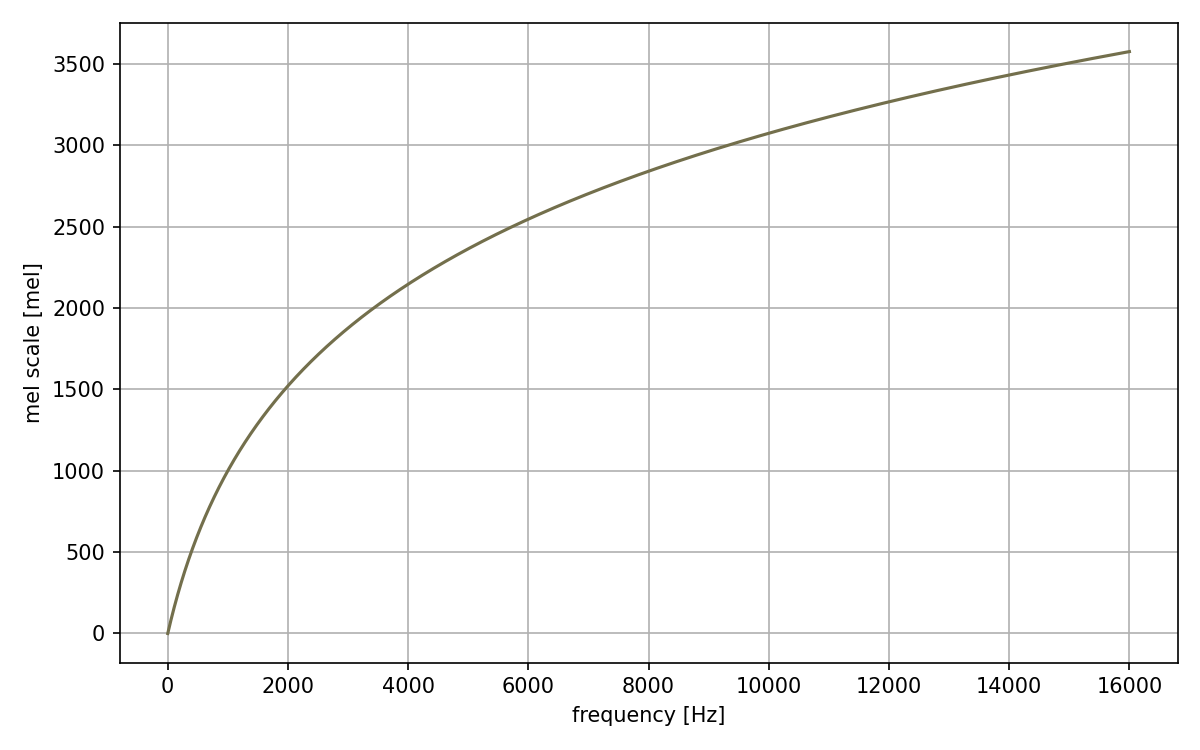
\includegraphics[width=0.40\textwidth]{./3_signal/figs/signal_mfcc_mel_scale}
  \caption{Mel scale as function of the frequency in a range of [0, \SI{16}{\kilo\hertz}].}
  \label{fig:signal_mfcc_mel_scale}
\end{figure}
\FloatBarrier
\noindent
The Mel and frequency window functions or equidistant mel filter bands are shown in \rfig{filter_bands}.
\begin{figure}[!ht]
  \centering
  \subfigure[mel space]{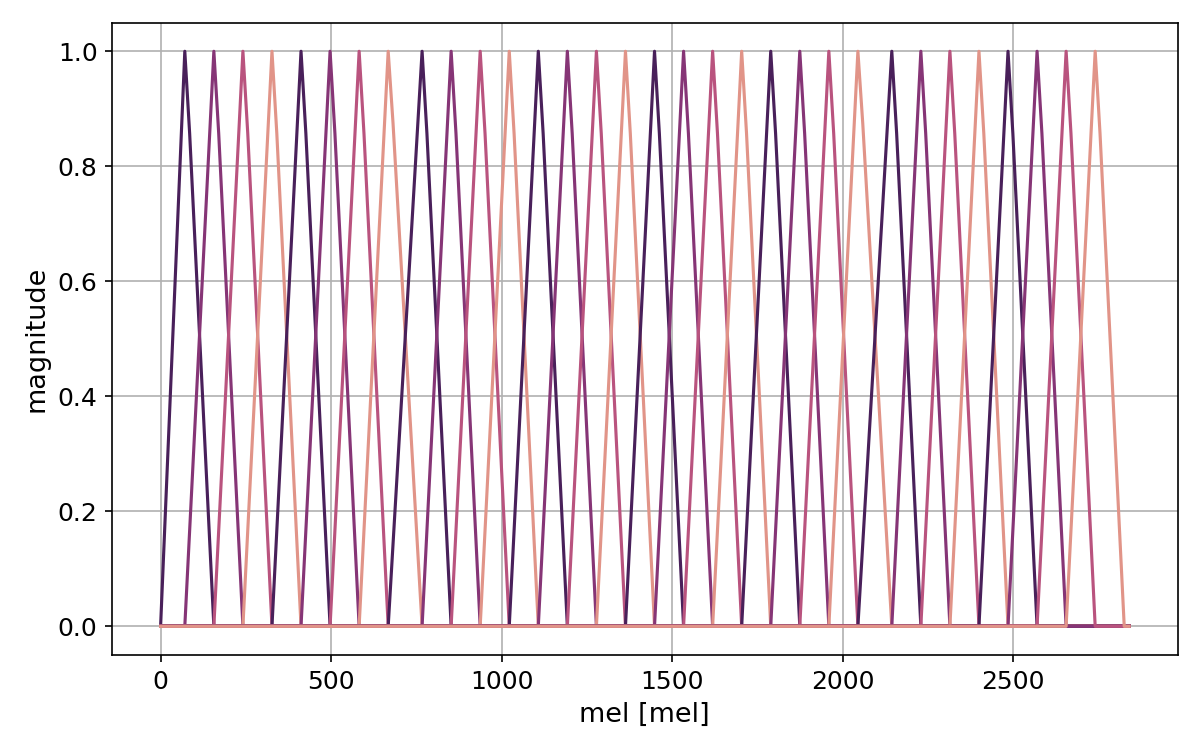
\includegraphics[width=0.40\textwidth]{./3_signal/figs/signal_mfcc_weights_mel}}
  \quad
  \subfigure[frequency space]{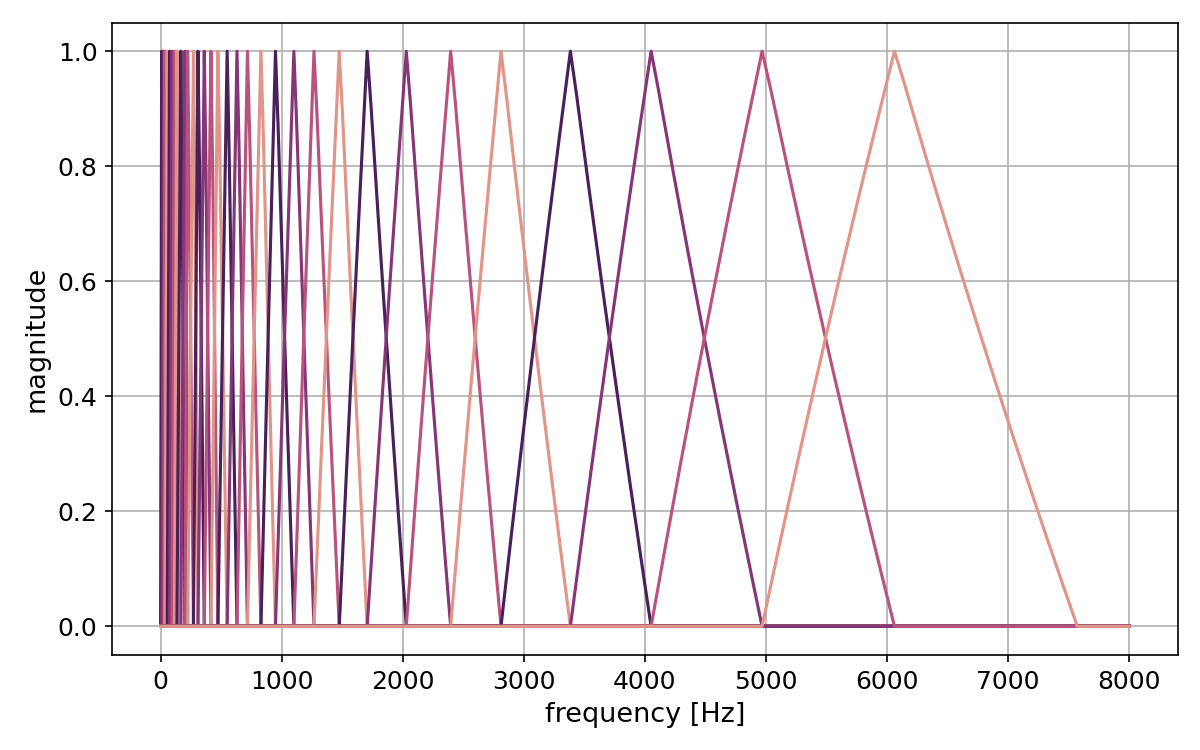
\includegraphics[width=0.40\textwidth]{./3_signal/figs/signal_mfcc_weights_f}}
  \caption{Equidistant Mel filter bands with a total number of 32 bands.}
  \label{fig:filter_bands}
\end{figure}
\FloatBarrier
\noindent
The creation of those filter bands is not described mathematically, because the graphical showcase is much more intuitive and easier to understand, but for further calculations those filter bands are notated in a weight matrix called $W_m \in \R^{B \times N}$, where $B$ are the amount of used filter bands as rows and $N$ the amount of frequency / mel bins of the DFT transformed and windowed input signal as columns in the matrix.

% dct
The DCT is very similar to the Fourier transform and projects the input signal to a set of orthogonal basis functions, but outpus only real valued signals instead of complex ones.
Different types of DCTs formulations exists, but most commonly the \enquote{type 2} DCT is used and calculated as:
% dct
\begin{equation}\label{eq:signal_mfcc_dct}
  X[c] = \sum_{n=0}^{N-1} x[n] \, \cos{\left[ \frac{\pi}{N} \left( n + \frac{1}{2} \right) c \right]}
\end{equation}
with $c$ as cepstrum index and $n$ as sample index of a signal with total length of $N$.
This can be conveniently written in matrix notation with a total number of $C$ cepstral coefficients:
% dct matrix
\begin{equation}\label{eq:signal_mfcc_dct_matrix}
  X =  x \, \mathcal{D} \quad \mathrm{with} \quad \mathcal{D}[n, c] = \cos{\left[ \frac{\pi}{N} \left( n + \frac{1}{2} \right) c  \right]}, 
  \quad n, c = (0, 1 \dots N - 1), (0, 1 \dots C) 
\end{equation}
with $\mathcal{D} \in \R^{N \times C}$ as DCT matrix and input signal $x \in \R^N$ which gives the transformed signal $X \in \R^C$
The DCT basis functions illustrated in a matrix in two different color schemes are shown in \rfig{signal_mfcc_dct}.
\begin{figure}[!ht]
  \centering
  \subfigure[DCT with continuous color scheme]{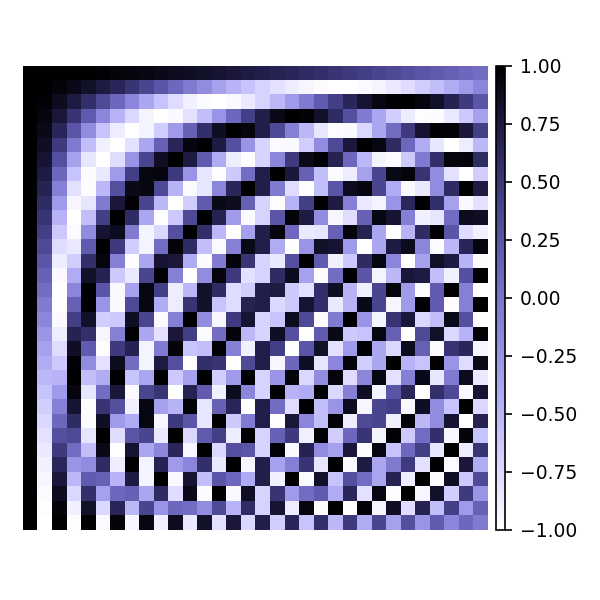
\includegraphics[width=0.35\textwidth]{./3_signal/figs/signal_mfcc_dct}}
  \quad
  \subfigure[DCT with diverging color scheme]{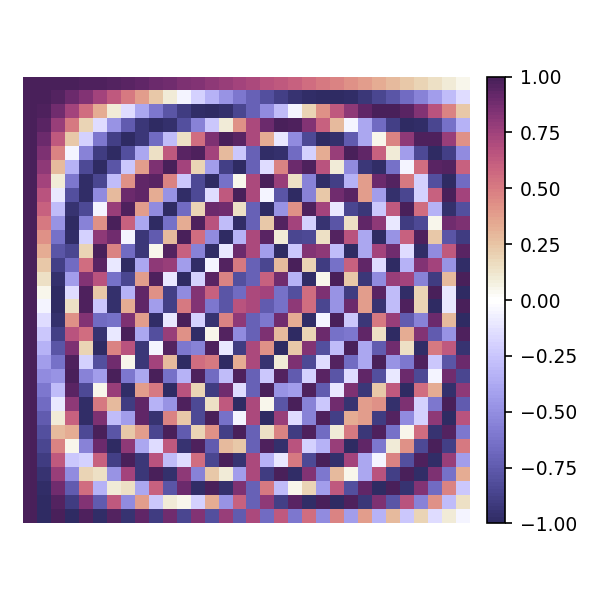
\includegraphics[width=0.35\textwidth]{./3_signal/figs/signal_mfcc_dct-div}}
  \caption{DCT matrix with 32 basis functions illustrated with a continuous and a diverging color scheme.}
  \label{fig:signal_mfcc_dct}
\end{figure}
\FloatBarrier
\noindent
The MFCCs $U \in R^{M \times C}$ are calculated from the log scaled power spectrum of the STFT $\tilde{X} \in \C^{M \times N}$ computed in \req{signal_spec_stft_matrix}, the filter band weights collected in the matrix $W_m \in \R^{B \times N}$ and transformed with the DCT matrix $\mathcal{D} \in R^{B \times C}$ as following:
\begin{equation}
    U = \log{ \left[ \, \abs{\tilde{X}}^2 \, W_m^T \, \right] } \, \mathcal{D}.
\end{equation}
Note that the rows represent all shifts with the hop size and the columns are the individual cepstral coefficients of $U$.
The parameters to choose from are therefore the amount of filter bands and the amount of cepstral coefficients.

Another important aspect is the visualization of MFCC features.
MFCCs computed as shown above, are not well intended for visualizations, because their individual coefficients value space differs strongly from each other.
For example the first coefficient equals a summation of all filter bands of the spectrogram and is therefore some kind of energy measure, while the other coefficients are different weighted sum combinations of the filter bands.
Further the most of the signal energy is located in the lower frequency bands, which impacts the value space of the coefficients with strongly weighted low frequency bands.
The differences in the value space leads to a problem in the visualization with a linear color scheme, so that some coefficients changes cannot be shown appropriately.
A solution to this problem is to normalize the feature vectors over each frame dimension with the infinity norm as:
% frame normalisation
\begin{equation}\label{eq:signal_mfcc_norm}
  \hat{U}[m, c] = \frac{U[m, c]}{\norm{u_c[m]}_\infty} \quad \forall m, c = (1, \dots, M), (1, \dots, C)
\end{equation}
where $m$ is again the frame (time) index, $c$ the individual MFCC coefficient and $u_c[m]$ the individual MFCC coefficient vector over all frames.
This equation gives a value space between $[0, 1]$ for each feature vector $u_c[m]$.

A visualization of MFCC features with 32 filter bands and 32 cepstral coefficients with frame based normalization of each coefficient is shown in \rfig{signal_mfcc_showcase_mfcc32}.
\begin{figure}[!ht]
  \centering
    \subfigure[left]{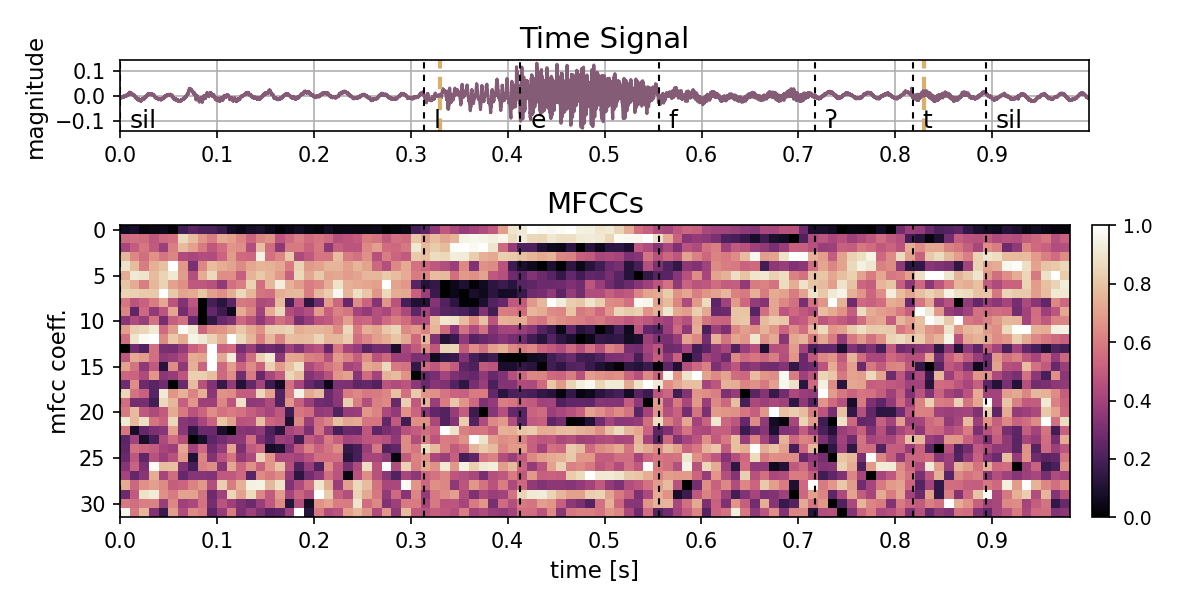
\includegraphics[width=0.45\textwidth]{./3_signal/figs/signal_mfcc_showcase_mfcc32_left0}}
    \subfigure[right]{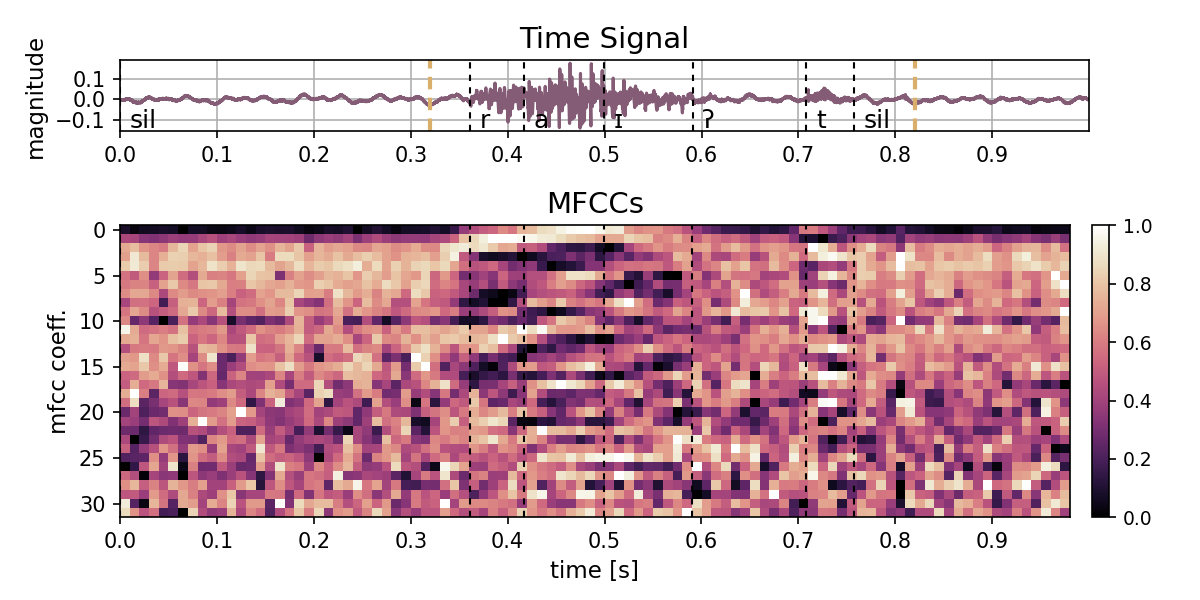
\includegraphics[width=0.45\textwidth]{./3_signal/figs/signal_mfcc_showcase_mfcc32_right0}}
    \subfigure[up]{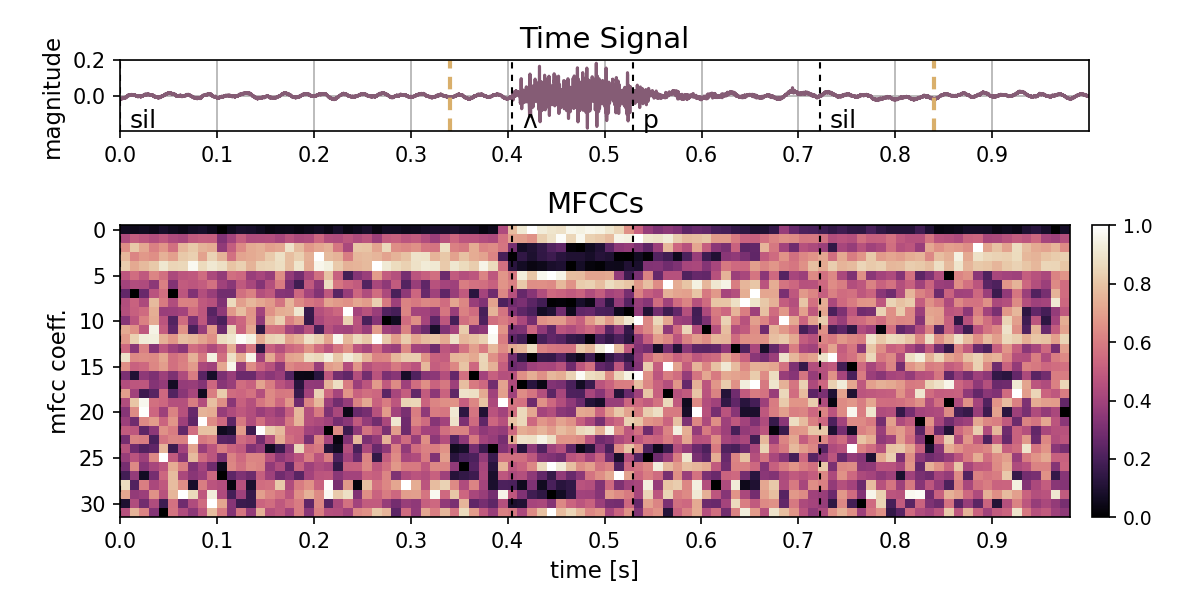
\includegraphics[width=0.45\textwidth]{./3_signal/figs/signal_mfcc_showcase_mfcc32_up0}}
    \subfigure[down]{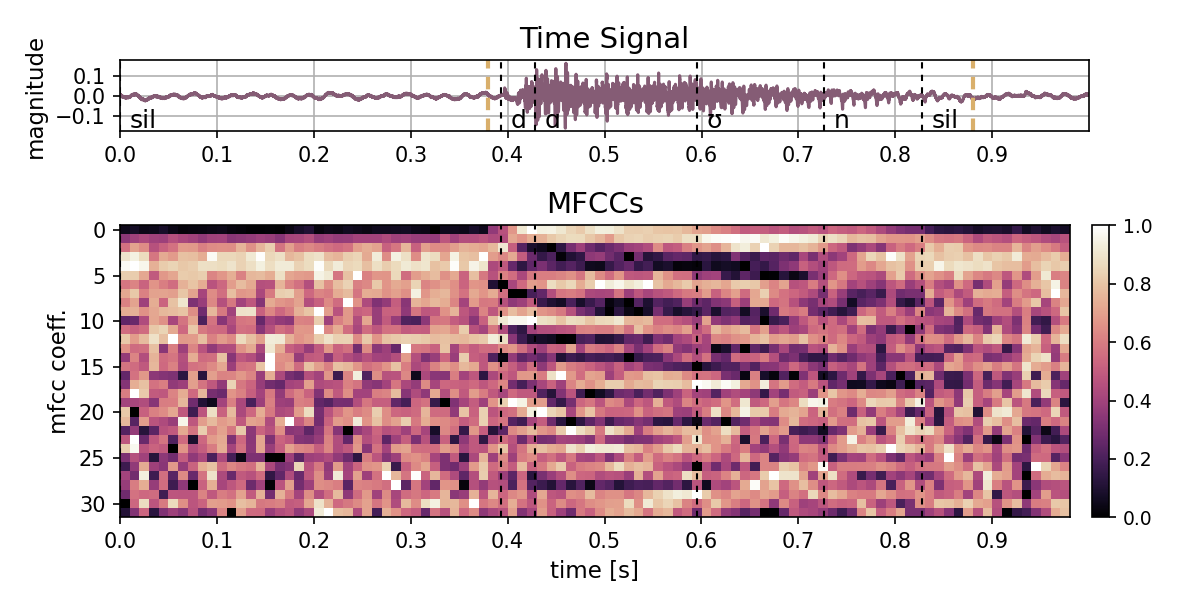
\includegraphics[width=0.45\textwidth]{./3_signal/figs/signal_mfcc_showcase_mfcc32_down0}}
    \subfigure[go]{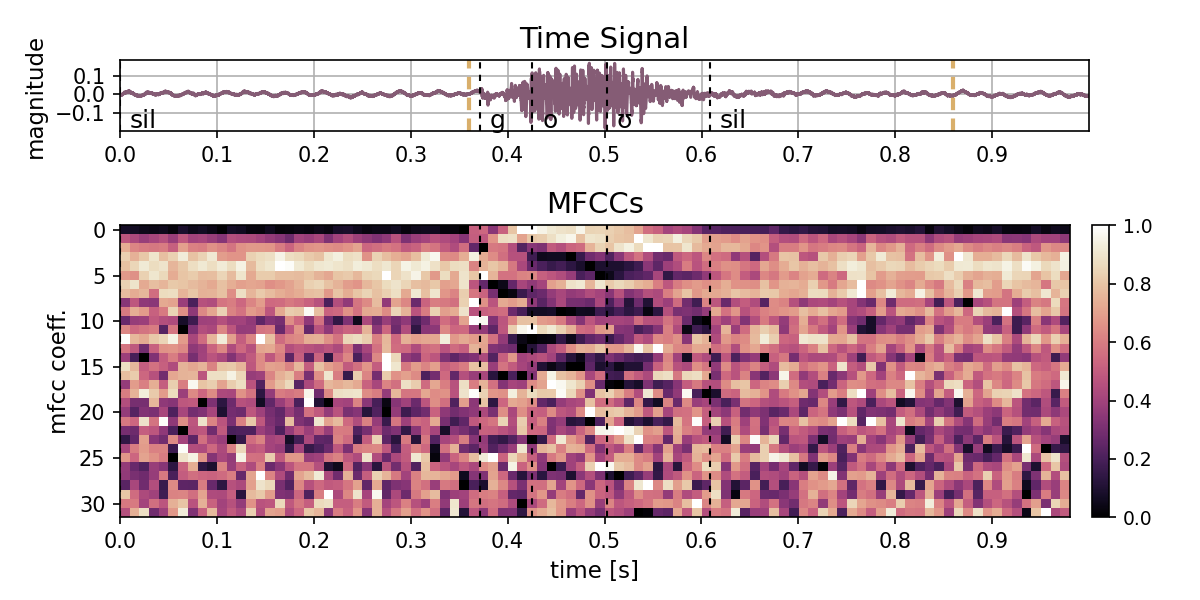
\includegraphics[width=0.45\textwidth]{./3_signal/figs/signal_mfcc_showcase_mfcc32_go0}}
  \caption{MFCC with 32 filter bands and 32 cepstral coefficients visualized with frame-based normalization.}
  \label{fig:signal_mfcc_showcase_mfcc32}
\end{figure}
\FloatBarrier
\noindent
The frame based normalization is an interesting aspect to improve the visualization of the MFCC features, however it can be critical. 
A normalization changes important structures within the feature space and it cannot be answered yet if this is a problem for neural networks or degrades the classification performance.
One more research question arises here: Is it possible to use frame based normalized MFCC features as inputs to neural networks and what are the results to the accuracy and training of the models.


% --
% enhancement

\subsection{MFCC Feature Usage and Enhancement}\label{sec:signal_mfcc_enhancement}
After the MFCCs are computed with the choice of filter bands $B$ and cepstral coefficients $C$, they can already be used as input features for neural networks.
The question arises, whether a further feature enhancement can be done to improve the performance in classification.
The best practice, used in many papers, is to apply $B=32$, $C=12$, compute derivatives of those 12 MFCC coefficients named as deltas and double deltas (second derivative) and add energy vectors of the 12 coefficients and the deltas.
The deltas are simply computed as frame $m$ difference of the MFCCs with:
\begin{equation}\label{eq:signal_mfcc_delta}
  \Delta u_i[m] = \frac{u_i[m - 1] + u_i[m + 1]}{2}
\end{equation}
where $u_i \R^M$ is the i-th MFCC coefficient vector and $m$ the frame index.
Note that the edges of the delta computations at $m=0$ and $m=M$ are not computed and the same value is obtained from the neighbour.
The second derivative of MFCC features, known as double deltas, are then the frame differences of the deltas, similar to \req{signal_mfcc_delta}
An energy feature vector can be computed from each of the MFCCs, deltas and double deltas by its own, with for instance simply:
\begin{equation}
  e[m] = u[m] \, u[m]^T 
\end{equation}
where $u[m] \in \R^C$ is the MFCC feature vector of frame $m$.

The MFCCs, their deltas and double deltas and energy vectors can then be simply stacked at top of each other and used as enhanced inputs to neural networks.
In this thesis the feature vectors are stacked as following:
\begin{enumerate}
    \item 12 MFCCs
    \item 1 Energy feature of the 12 MFCCs
    \item 12 Deltas
    \item 1 Energy feature of the 12 Deltas
    \item 12 Double Deltas
    \item 1 Energy feature of the 12 Double Deltas
\end{enumerate}
which sums up to a 39-dimensional feature vector, very commonly used in the literature.
Many papers do not explicitly explain how the 39 MFCCs are calculated in detail, in most cases however this constellation is applied.
The computation of 39 MFCCs are shown in \rfig{signal_mfcc_showcase_mfcc39}
\begin{figure}[!ht]
  \centering
    \subfigure[left]{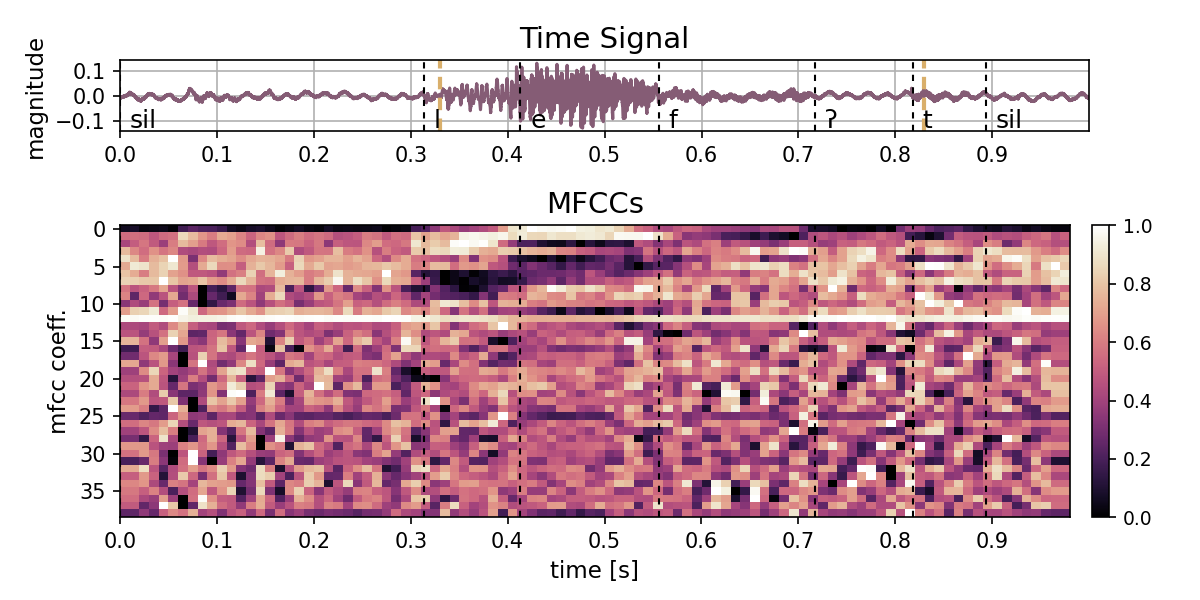
\includegraphics[width=0.45\textwidth]{./3_signal/figs/signal_mfcc_showcase_mfcc39_left0}}
    \subfigure[right]{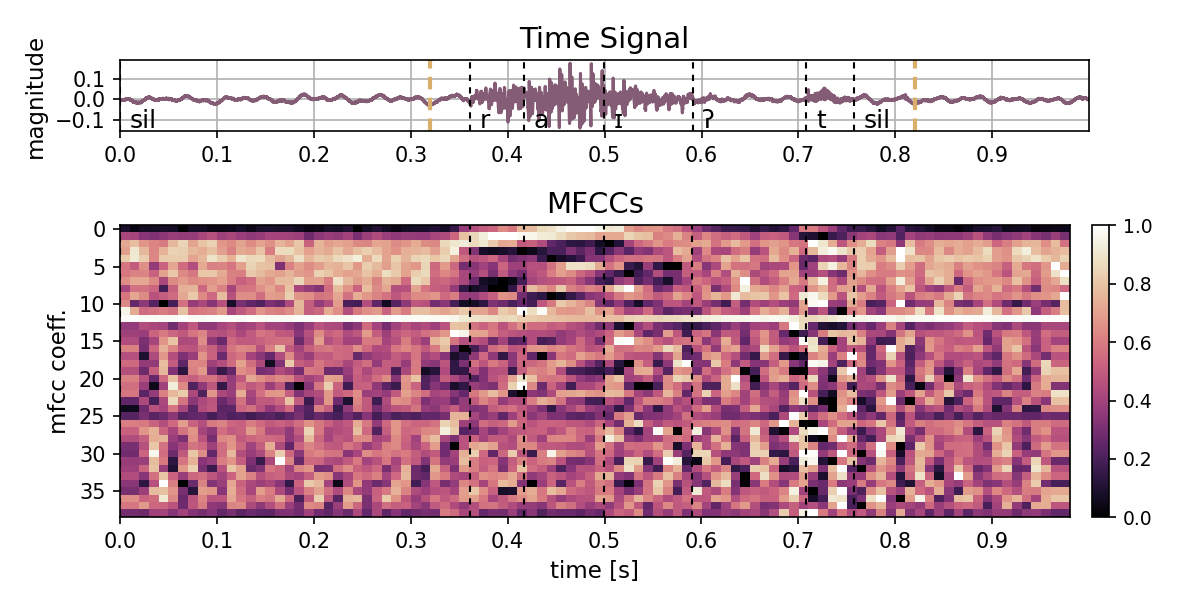
\includegraphics[width=0.45\textwidth]{./3_signal/figs/signal_mfcc_showcase_mfcc39_right0}}
    \subfigure[up]{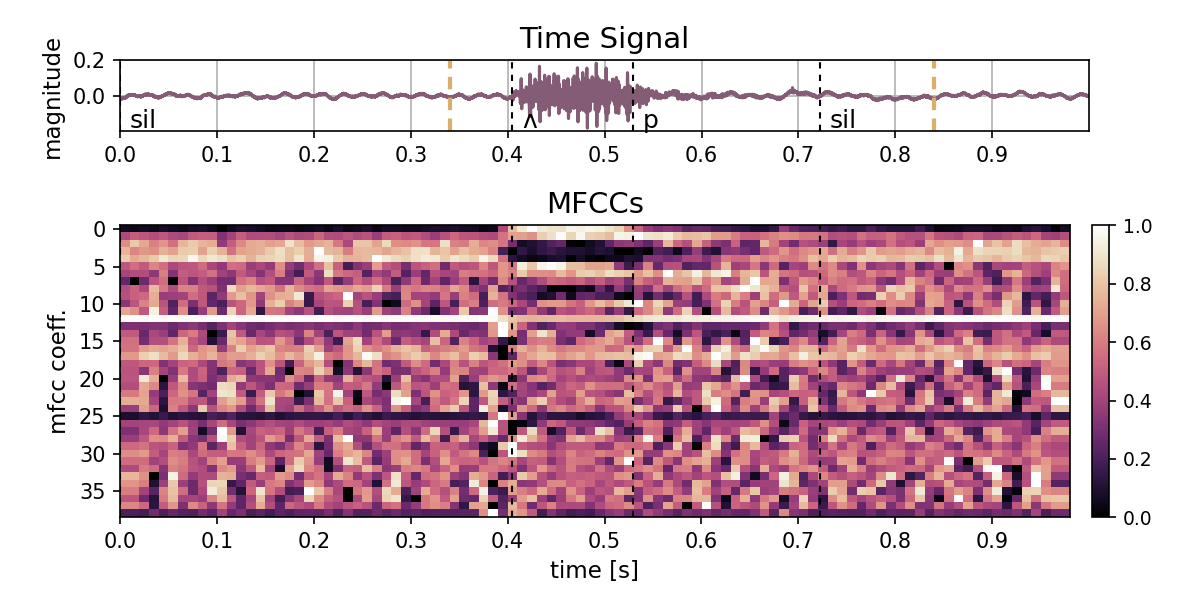
\includegraphics[width=0.45\textwidth]{./3_signal/figs/signal_mfcc_showcase_mfcc39_up0}}
    \subfigure[down]{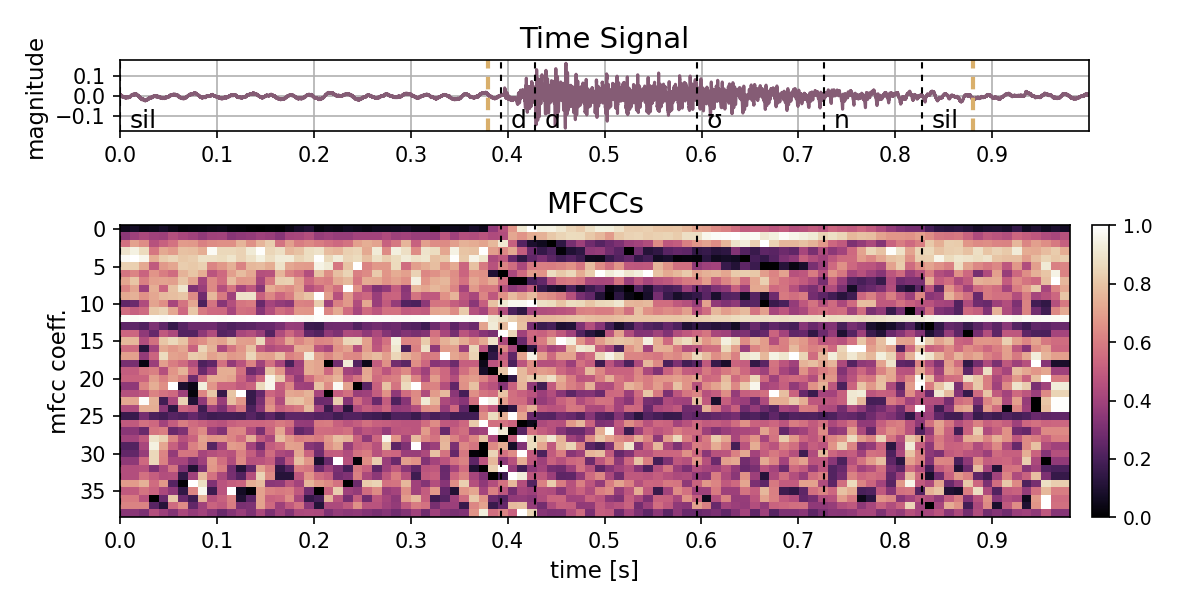
\includegraphics[width=0.45\textwidth]{./3_signal/figs/signal_mfcc_showcase_mfcc39_down0}}
    \subfigure[go]{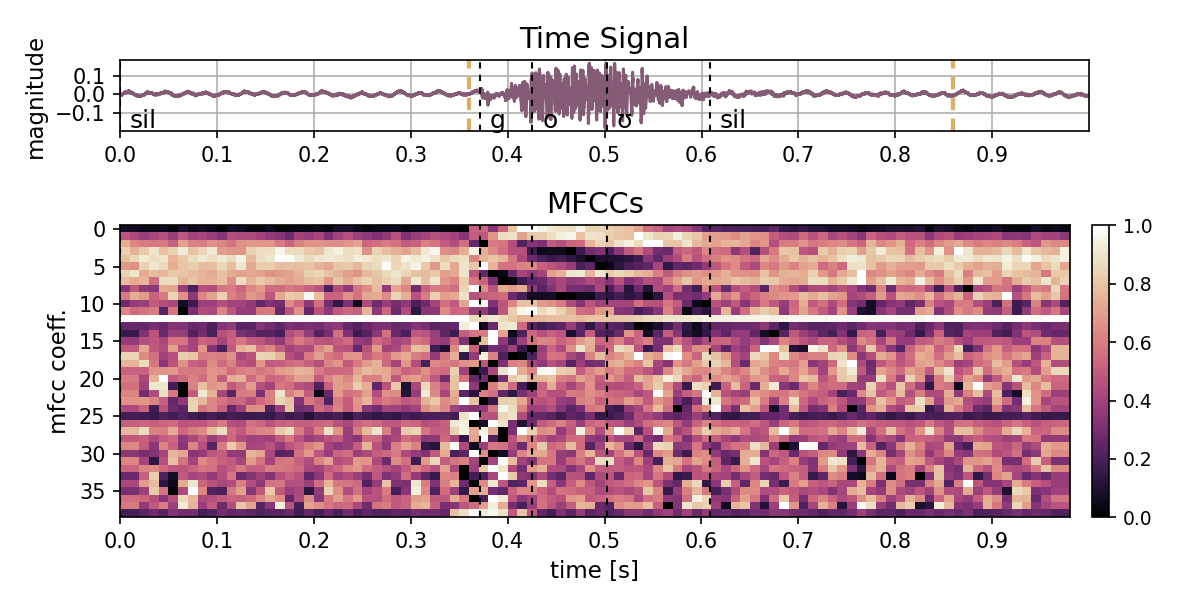
\includegraphics[width=0.45\textwidth]{./3_signal/figs/signal_mfcc_showcase_mfcc39_go0}}
  \caption{MFCC with 32 filter bands and 12 cepstral coefficients, deltas, double deltas and energy vector visualized with frame-based normalization.}
  \label{fig:signal_mfcc_showcase_mfcc39}
\end{figure}
\FloatBarrier
\noindent

% --
% energy consumption

\subsection{Energy consumption}
The energy consumption is evaluated on the operations needed to process a \SI{500}{\milli\second} time signal sampled with $f_s = \SI{16}{\kilo\hertz}$ to MFCCs.
The computation of a DFT with $N$ Fourier coefficients is...



% --
% visualization

%\subsection{Visualization of MFCC features}\label{sec:signal_mfcc_visualization}


%To show this difference in value space in a negative example in practice, the MFCCs of the self-recorded speech command waveform \enquote{left0.wav} is shown in \rfig{left0_mfcc_only}.
% useless
% \begin{figure}[!ht]
%   \centering
%     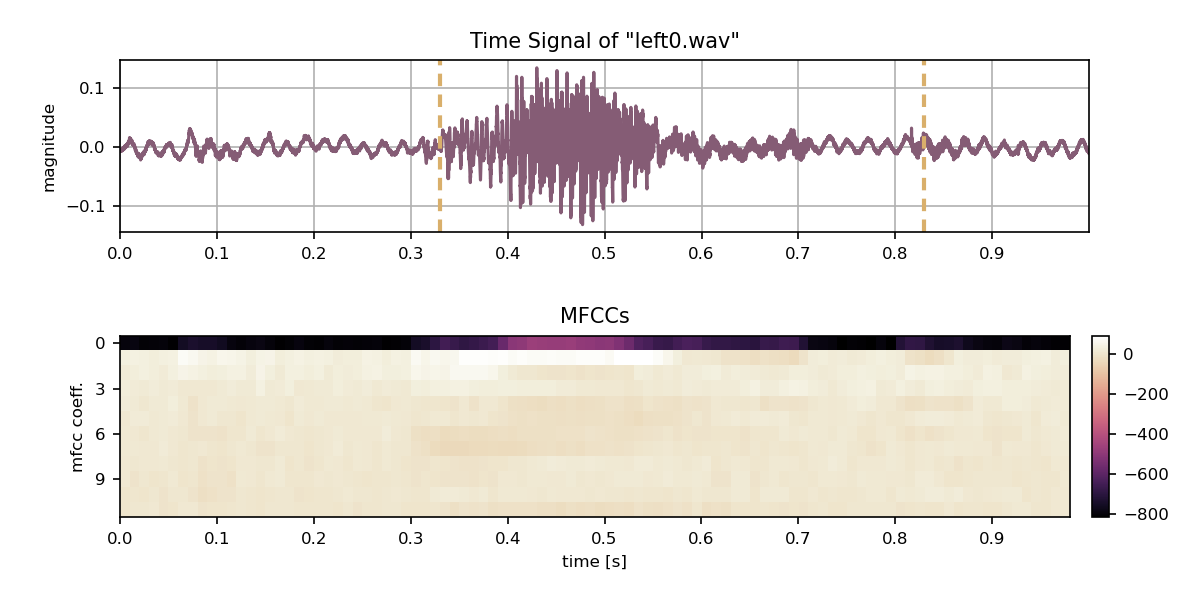
\includegraphics[width=0.75\textwidth]{./3_signal/figs/signal_mfcc_left0_mfcc_only.png}
%   \caption{Bad visualisation of the 12 MFCCs features extracted from \enquote{left0.wav}.}
%   \label{fig:left0_mfcc_only}
% \end{figure}
% \FloatBarrier
% \noindent
% Not much structure of the MFCCs can be seen here, due to the vast value difference of the first coefficient. At least the first coefficient shows, where the center of signal energy is placed on the time scale, but other than that, this visualisation is worthless.
% Another very bad visualisation is shown by computing the 39 MFCC feature vectors (with Deltas, Double Deltas and Energies) in \rfig{left0_no_order}.

% \begin{figure}[!ht]
%   \centering
%     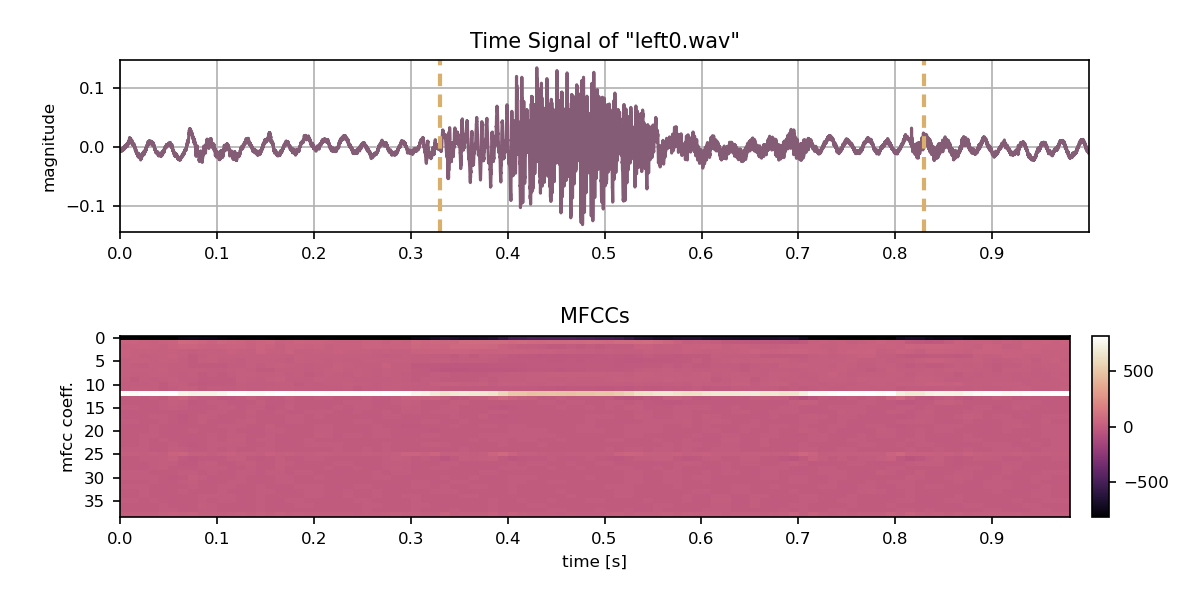
\includegraphics[width=0.75\textwidth]{./3_signal/figs/signal_mfcc_left0_no_order_norm0.png}
%   \caption{Very bad visualisation of 39 MFCC features extracted from \enquote{left0.wav}.}
%   \label{fig:left0_no_order}
% \end{figure}
% \FloatBarrier
% \noindent
% There appears an even greater gap of different value spaces and even less is seen.

% One solution is to show the features in different value groups. 
% For instance putting the first coefficient and its deltas is in one group, the other coefficients in another and their deltas and energies as well in own groups. 
% Now it is possible to observe some structure in the visualizations, with an example shown in \rfig{left0_order}.

% \begin{figure}[!ht]
%   \centering
%     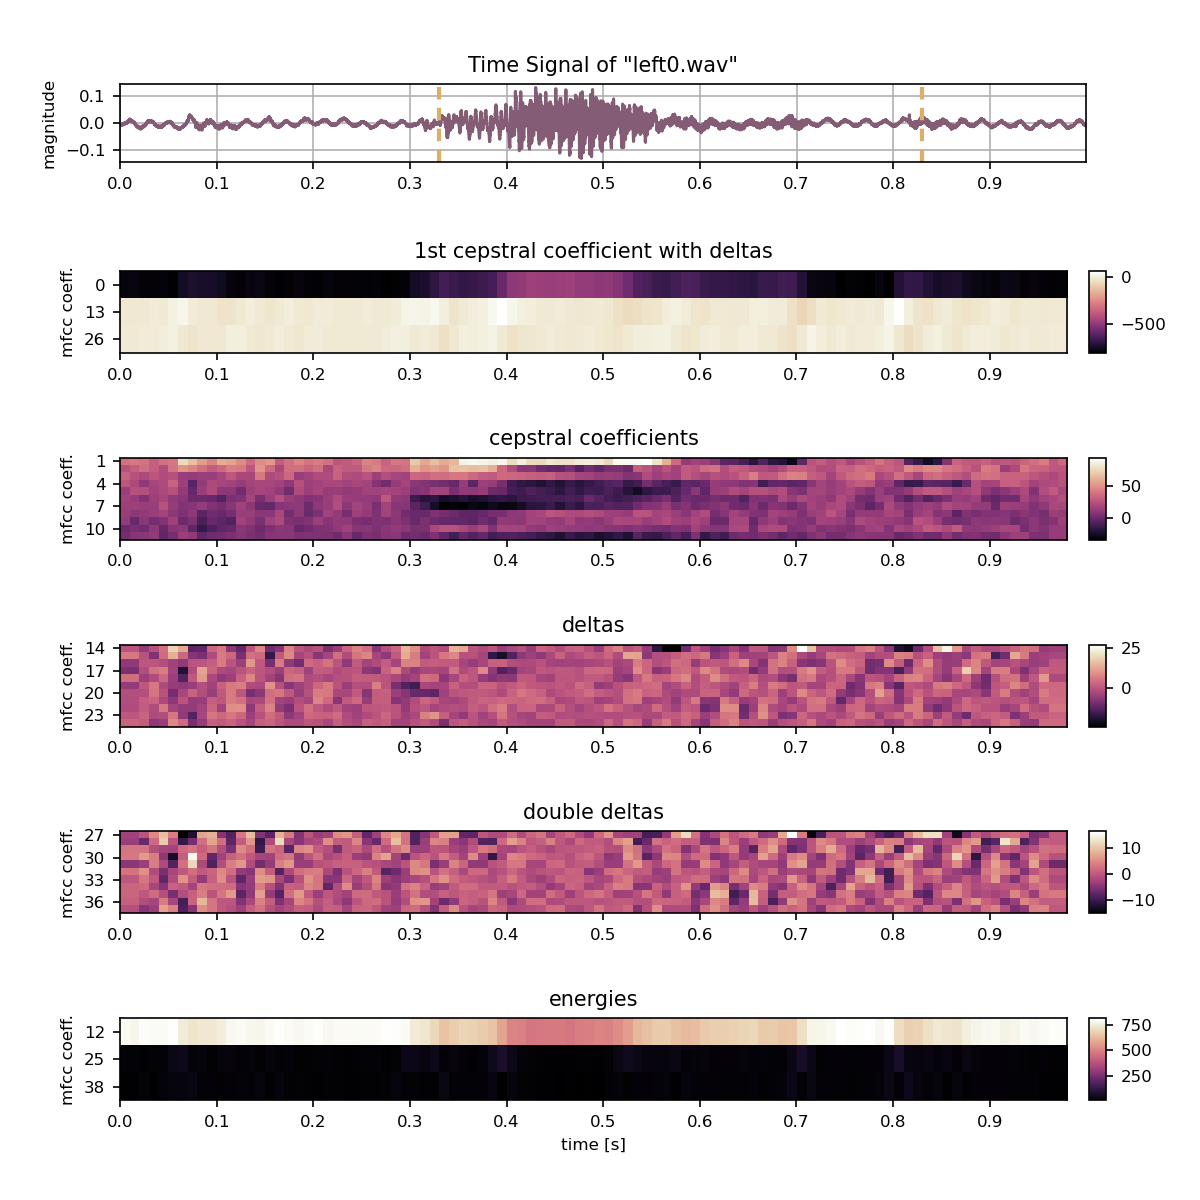
\includegraphics[width=0.75\textwidth]{./3_signal/figs/signal_mfcc_left0_norm0.png}
%   \caption{Good visualisation of 39 MFCC features extracted from \enquote{left0.wav} with own value groupings.}
%   \label{fig:left0_order}
% \end{figure}
% \FloatBarrier
% \noindent
% Another way to improve the visualization is to normalize the feature vectors over each frame dimension with the infinity norm as:

% % frame normalisation
% \begin{equation}\label{eq:signal_mfcc_norm}
%   \hat{U}[m, l] = \frac{U[m, l]}{\norm{u_l[m]}_\infty}
% \end{equation}
% where $m$ is again the variable in frames, $l$ the individual MFCC coefficient and $u_l[m]$ the individual MFCC coefficient vector over all frames.
% This equation gives a value space between $[0, 1]$ for each feature vector $u_l[m]$.

% A visualization with frame normalization of the 39 MFCC feature vectors of \enquote{left0.wav} is shown in \rfig{left0_order},

% \begin{figure}[!ht]
%   \centering
%     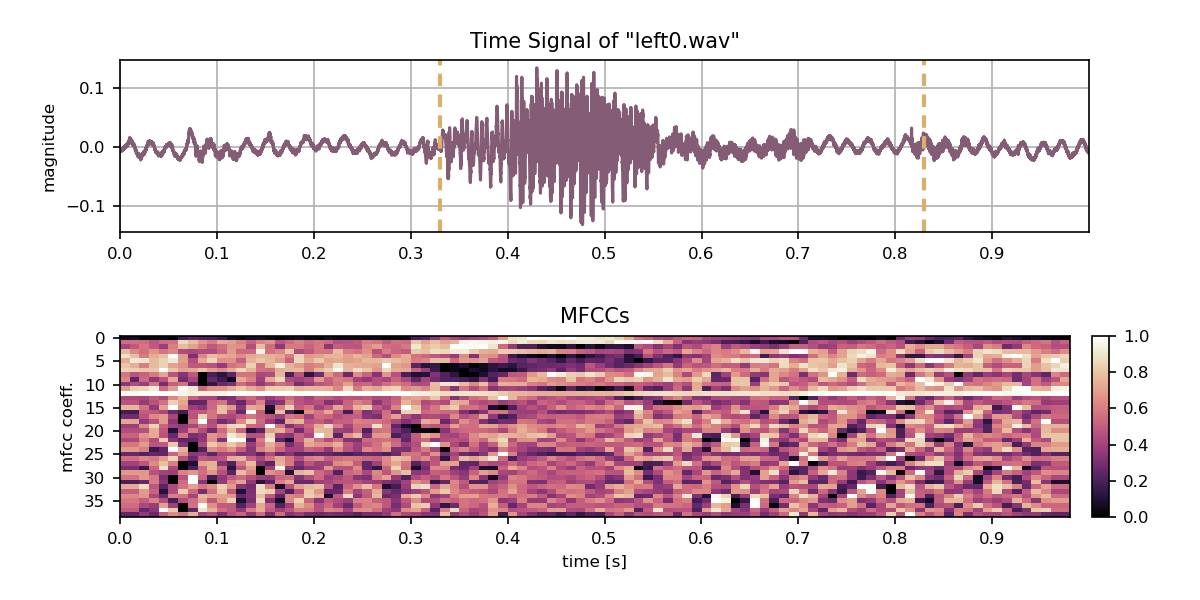
\includegraphics[width=0.75\textwidth]{./3_signal/figs/signal_mfcc_left0_no_order_norm1.png}
%   \caption{Normalization of 39 MFCC features extracted from \enquote{left0.wav}.}
%   \label{fig:left0_no_order_norm1}
% \end{figure}
% \FloatBarrier
% \noindent
% or in an even better one shown in \rfig{left0_order_norm1}.

% \begin{figure}[!ht]
%   \centering
%     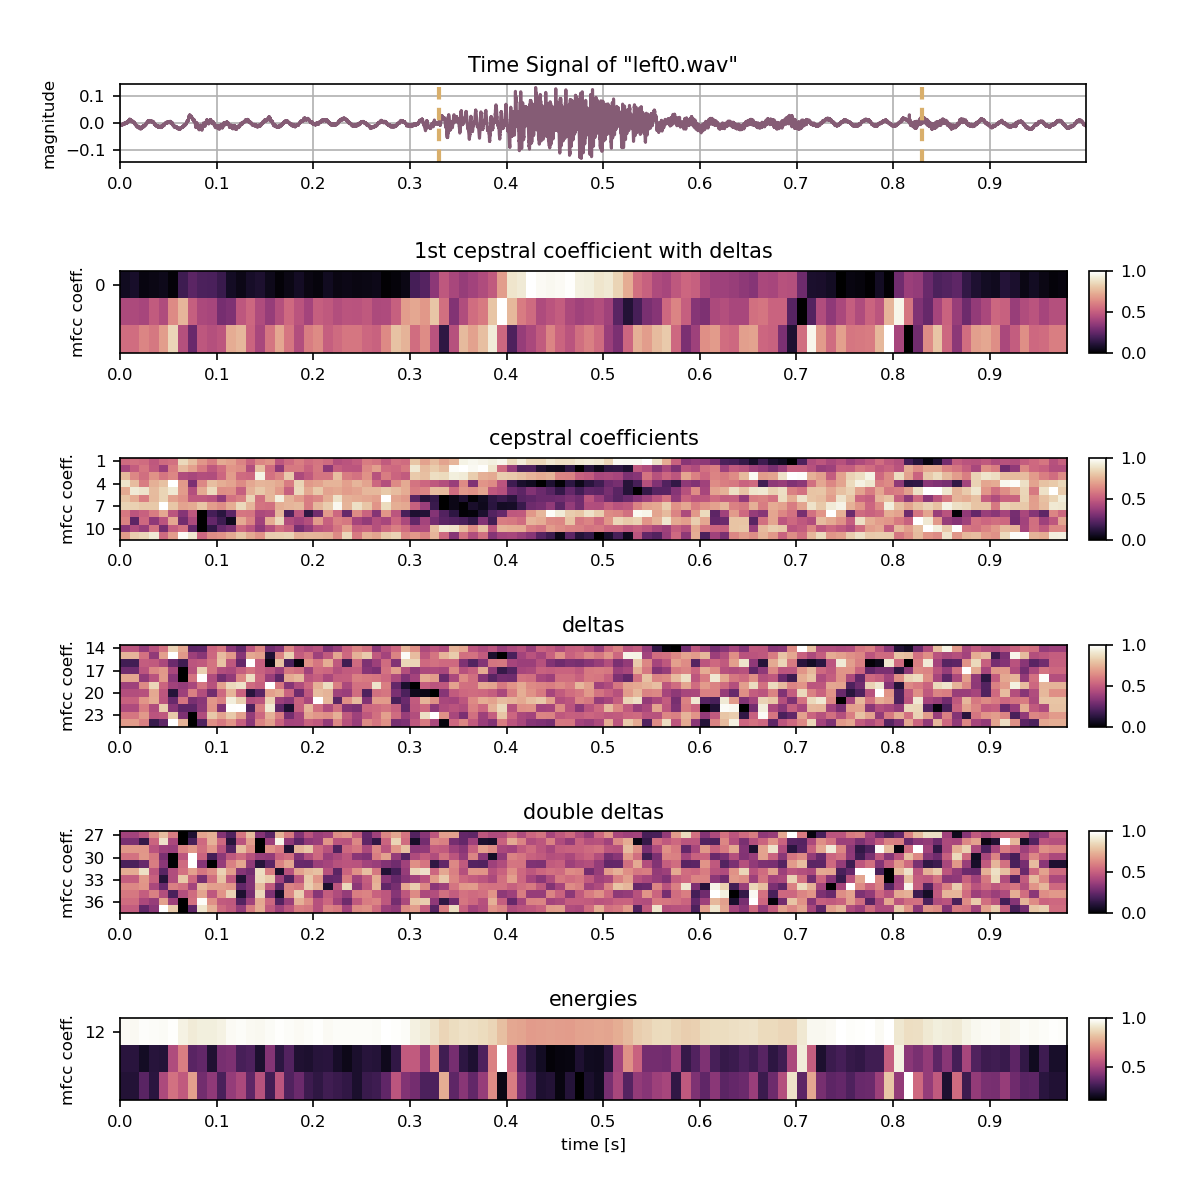
\includegraphics[width=0.75\textwidth]{./3_signal/figs/signal_mfcc_left0_order_norm1.png}
%   \caption{Normalisation of 39 MFCC features extracted from \enquote{left0.wav} with groups.}
%   \label{fig:left0_order_norm1}
% \end{figure}
% \FloatBarrier
% \noindent
